\documentclass[tikz]{standalone}
\usepackage{bm}
\begin{document}
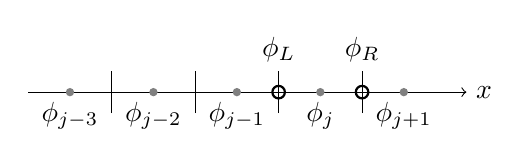
\begin{tikzpicture}[
  scale=0.53,
  cpnt/.style={fill=gray},
]

\draw [->] (-5,0) -- (5.5,0) node [right] {$x$};
\draw (-3,-0.5) -- (-3,0.5);
\draw (-1,-0.5) -- (-1,0.5);
\draw (1,-0.5) -- (1,0.5) node [above] {$\phi_L$};
\draw (3,-0.5) -- (3,0.5) node [above] {$\phi_R$};

\path [cpnt] (-4,0) circle [radius=0.1] node [below] {$\phi_{j-3}$};
\path [cpnt] (-2,0) circle [radius=0.1] node [below] {$\phi_{j-2}$};
\path [cpnt] (0,0) circle [radius=0.1] node [below] {$\phi_{j-1}$};
\path [cpnt] (2,0) circle [radius=0.1] node [below] {$\phi_j$};
\path [cpnt] (4,0) circle [radius=0.1] node [below] {$\phi_{j+1}$};
\draw [thick] (1,0) circle [radius=0.15];
\draw [thick] (3,0) circle [radius=0.15];

\end{tikzpicture}
\end{document}
